\chapter{Génération d'une \bdd}
  \section{Déclaration et paramétrage d'un objet \IGEN }
    \subsection{Constructeur}\label{Constructeur}
      Il existe deux constructeurs à la classe \IGEN:
      \begin{itemize}
       \item Constructeur par défaut:\\              
       \vspace{0.3cm}
       \hspace{0.3cm} \Cpp{\IGEN\ obj\_igen;}
       
       \item Constructeur avec arguments: \\
       permet de créer un objet de la classe \IGEN\ en lui spécifiant la méthode et la référence utilisée:
       
       \vspace{0.3cm}
       
	\hspace{0.3cm}\Cpp{\IGEN\ obj\_igen(\str{EOS\_Refprop}, \str{Water});}
	
	
      \end{itemize}
      
      \subsection{Paramètres}\label{parametres}
	\subsubsection{Méthode et référence}\label{metetref}
      
	 Comme pour tout objet \EOS, il est nécessaire d'affecter à un objet de la classe \IGEN\
	 une méthode ainsi qu'une référence. Ceci peut être fait à partir des méthodes 
	 \Cpp{set\_method} et \Cpp{set\_reference} ou directement à la création de l'objet 
	 (Cf. paragraphe \ref{Constructeur}). Ces 2 paramètres définissent l'objet de la classe \EOS\
	 (attribut \Cpp{fluid} de la classe \IGEN) avec lequel sera calculé les propriétés physiques, puis généré la \bdd.
	 
	 \subsubsection{Bornes de la \bdd}\label{bornes}
	 
	 Avant la création du maillage, il est nécessaire de définir les limites en pression et en température, du domaine de la \bdd\ 
	 (pression min, pression max, température min et température max). 
	 Ces paramètres doivent être affectés à l'aide de la méthode \Cpp{set\_extremum} de la classe \IGEN.
	 Ces données, ensuite, sont traduites, afin que le maillage dépende de la \underline{pression} et de l'\underline{enthalpie}. 
	 
	 	 
	 
	 \subsubsection{Initialisation du maillage}\label{initm}
	 
	 Le maillage doit être initialisé à partir de la méthode \Cpp{make\_mesh}, possédant 3 paramètres:
	 \vspace{0.3cm}
	 \begin{itemize}
	  \item nombre de \n s en pression (obligatoire);
	  \item nombre de \n s en enthalpie (obligatoire);
	  \item niveau de raffinement maximal (optionnel).
	 \end{itemize}
	 \smallbreak
	 \vspace{0.5cm}
	 La routine \Cpp{make\_mesh} réalise les tâches suivantes:
	 \vspace{0.3cm}
	 \begin{itemize}
	  \item Calcul de l'enthalpie minimum et de l'enthalpie maximum du maillage;
	  \item Instanciation de 2 objets de la classe \MESH:
	  \begin{itemize}
	    \item[\ding{213}]Attribut \Cpp{mesh\_ph} de la classe \IGEN: maillage surfacique pression-enthalpie (\pph);
	    \item[\ding{213}]Attribut \Cpp{mesh\_p}  de la classe \IGEN: segment en pression (\sgp);
	  \end{itemize}
	  \item Création d'une \bdd\ temporaire;
	  \item Affectation de l'attribut \Cpp{obj\_Ipp} objet de la classe \EOS.
	 \end{itemize}
      
      \section{Critères de qualité}\label{qualite}
	\subsection{Déclaration}
	Les critères de qualité se définissent à l'aide de la méthode \Cpp{set\_quality}, via 4 paramètres:
	\vspace{0.3cm}
	\begin{itemize}
	 \item \Cpp{property}: propriété physique sur laquelle s'applique le critère de qualité;
	 \item \Cpp{type}: méthode de calcul de la qualité;
	 \item \Cpp{is\_abs}: norme définissant si la qualité est calculée en relatif ou en absolu\\ (0: relatif; 1: absolu);
	 \item \Cpp{limit\_qi}: Limite haute (seuil de qualité) que doit respecter l'écart entre
	 les calculs de la propriété avec l'interpolateur (\IPP) et les calculs de la propriété avec la méthode \EOS\ de référence.
	\end{itemize}
	\smallbreak
	\vspace{0.5cm}
	Pour un maillage il peut y avoir un nombre indéfini de critères de qualité, 
	à chaque appel de la méthode \Cpp{set\_quality} un nouvel objet de la classe \QI\ est créé, puis ajouté à 
	l'attribut \Cpp{qualities} de la classe \IGEN.
	
	
      \subsection{Principe}
      
      Les critères de qualité sont ce qui permet d'accorder la validité d'une maille
      ainsi que le maillage dans ça globalité.
      La qualité d'un maillage est estimée à l'aide de la méthode \Cpp{compute\_qualities} de la classe \IGEN.
      
      \subsubsection{calcul de la qualité}
      
      La qualité s'applique maille/maille, de façon indépendante.
      Ce sont les critères de qualité qui vont, dans le cas d'un raffinement
      local \para{raflocal}, déterminer si la maille a besoin d'être raffinée.
      \smallbreak\vspace{0.3cm}
      Aujourd'hui, pour calculer la qualité des mailles, une seule méthode est implémentée.
      La méthode se détermine, en affectant le mot clé \str{centre} au paramètre \Cpp{type},
      celui-ci indique que la propriété est calculée, via l'interpolateur et via la méthode de référence,
      au centre de la maille. Puis la différence de ces deux résultats est comparée au seuil, si elle est inférieure la maille
      est dite valide (en erreur sinon). En relatif la différence est divisée par le résultat de la méthode de référence.

      
      \subsubsection{Implémentation future}
      \begin{enumerate}
       \item D'autre méthodes de calcul de la qualité pourront être implémentées:
       \vspace{0.3cm}
       \begin{itemize}
	 \item \str{multipoint}: écart entre une grandeur interpolée et la grandeur d’origine en 9 points des mailles;
	 \item \str{d\_rho}: écart entre dérivée numérique de la masse volumique à partir des grandeurs interpolées et la valeur interpolées;
	 \item \str{d\_h}: écart entre la dérivée numérique de l’enthalpie en fonction de la température à pression constante.
       \end{itemize}
       \item Un calcul \EOS\ peut retourner une erreur, pour différentes raisons, celles-ci ne sont pas décrites ici.  
	Il est donc, possible que certains \n s d'un maillage soient dans un domaine ``non valide''.
	Ainsi, lorsqu'une maille a ces quatre \n s dans un domaine ``non valide'', il n'y aucune nécessité de la raffiner, 
	la validité des \n s pourrait être un paramètre de la validité de la maille.
      \end{enumerate}
	 
    \section{Raffinement}\label{raf}
    
    Deux types de raffinement sont implémentés dans la classe \IGEN, le raffinement global et le raffinement local. 
    Un raffinement s'arrête lorsque toutes les mailles sont valides \para{qualite}
    ou que son niveau maximum de raffinement est atteint \para{initm}.
    
    \subsection{Raffinement global}
    Le raffinement global permet, lorsqu'un critère de qualité n'est pas respecté de raffiner le maillage dans sa globalité (méthode \Cpp{make\_global\_refine}).
    Ainsi, par niveau de raffinement, chaque maille est divisée en quatre parties égales. 
    Cette méthode est peu optimisée car lorsqu'une seule maille est en erreur tout le maillage est raffiné.
    
    \subsection{Raffinement local}\label{raflocal}
    
    Le raffinement local a été implémenté dans le but de raffiner seulement les mailles dont les critères de qualité ne sont pas respectés.
    Cependant la démarche d'un raffinement local pose un problème de continuité des valeurs dans le \pph, en effet une propriété calculée à la 
    frontière de 2 mailles côte à côte, de taille différente, peut ne pas donner le même résultat d'une maille à l'autre (Cf Annexe \ref{cnt}). 
      
      \subsubsection{Principe}
      Le raffinement se réalise via la méthode \Cpp{make\_local\_refine} de la classe \IGEN.
      Cette méthode réalise les tâches suivante:
      \vspace{0.3cm}
      \begin{itemize}
       \item Calcul de la qualité: méthode \Cpp{compute\_qualities} de la classe \IGEN;
       \item Création des nouveaux \n s des maillages (\pph\ et \sgp): méthode \Cpp{add\_local\_nodes}, classe \MESH;
       \item Ajout des \n s de continuité (plan \textbf{ph}): méthode \Cpp{add\_continuity\_nodes}, classe \MESH;
       \item écriture d'une \bdd\ temporaire: méthode \Cpp{write\_tempory\_med}, classe \IGEN.
      \end{itemize}
      \vspace{0.5cm}
      
      \subsubsection{Création de \n s}
	\begin{description}
	 \item[\textbullet] \textbf{\sgp:}
	 \smallbreak
	 La réalisation d'un raffinement local, sur le \sgp, ne pose aucune difficulté:
	  \vspace{0.3cm}
	  \begin{itemize}
	  \item Ajout d'un point au centre des segments locaux dont la qualité n'est pas respecter;
	  \item renumérotation des \n s du \sgp\ global.
	  \end{itemize}
	 
	 \vspace{0.3cm}
	 \item[\textbullet] \textbf{\pph:}
	   \smallbreak
	   Pour effectuer un raffinement local, dans le \pph, deux types de maillage sont utilisés:
	   \vspace{0.3cm}
	   \begin{itemize}
	    \item maillage global: maillage fictif où toutes les mailles sont raffinées. 
	    Ce maillage est représenté par l'attribut \Cpp{node\_glb} qui décrit les \n s par un entier (Cf. Figure \ref{nodeglb}):
	      \begin{itemize}
		\item[\ding{213}] \Cpp{node\_glb[i] = 0}: \n s fictifs; 
		\item[\ding{213}] \Cpp{node\_glb[i] = 1}: \n s du maillage initial et \n s au centre d'une maille précédemment raffinée;
		\item[\ding{213}] \Cpp{node\_glb[i] = 2 ou 9}: \n s d'une maille raffinée, calculés sur un segment à \textbf{p} constant 
		(2: en cours de raffinement, 9: niveau de raffinement antérieur);
		\item[\ding{213}] \Cpp{node\_glb[i] = 3 ou 8}: \n s d'une maille raffinée, calculés sur un segment à \textbf{h} constant 
		(3: en cours de raffinement, 8: niveau de raffinement antérieur);
		\item[\ding{213}] \Cpp{node\_glb[i] = 4}: \n s au centre d'une maille en cours de raffinement;
	      \end{itemize}
	    \vspace{0.3cm}
	    \item maillage réel: maillage avec seulement les mailles en erreurs raffinées (maillage stocké dans la \bdd). 
	    Ici les \n s sont décrits par leurs valeurs en \textbf{p}, en \textbf{h} ainsi que leur type (Cf. \textbf{Continuité} paragraphe \ref{continuite}).
	   \end{itemize}

	 \begin{figure}[H]
	  \center
	  \includegraphics[width=0.75\textwidth]{schema_2d_ndglb.eps}
	  \caption{Exemple d'un maillage global, représentation graphique du vecteur \Cpp{node\_glb}}\label{nodeglb}
	 \end{figure}
	 
	 Le raffinement local dans le \pph, est réalisé selon l'algorithme suivant:
	 \vspace{0.3cm}
	 \begin{itemize}
	  \item Création de l'équivalence mailles globales - mailles réelles;
	  
	  \item Calculs du nombre de \n s et du nombre de mailles à ajouter pour ce niveau de raffinement;
	  
	  \item Détermination de la position des nouveaux \n s réels dans le maillage global;
	  
	  \item Affectation à chaque \n s des valeurs \textbf{h} et \textbf{p};
	  
	  \item Spécification du vecteur d'équivalence \n s globaux - \n s réel;
	  
	  \item Détermination de la correspondance des mailles globales aux 4 \n s qui l'entourent (attribut \Cpp{med\_to\_node} de la classe \MESH).
	 \end{itemize}

	 
	\end{description}

	Il est à noter qu'un critère de qualité avec une propriété calculée dans le \pph\ 
	impose un raffinement seulement dans le maillage \textbf{ph} 
	et respectivement pour une propriété du \sgp.

      
      \subsubsection{Continuité}\label{continuite}
      
      La continuité est construite à partir du maillage global, sur lequel sont ajoutés les \n s de continuité:
      \begin{itemize}
       \item placement des \n s existant (\n s de continuités et \n s réels) dans le nouveau maillage global;
        
       \item Affectation des valeurs \textbf{h} et \textbf{p} (Attribut \Cpp{continuity\_h} et \Cpp{continuity\_p}, de la classe \MESH)
       et ajout au maillage global des nouveaux \n s de continuité (Attribut \Cpp{continuity\_node} de la classe \MESH):
	\begin{itemize}
	\item[\ding{213}] \Cpp{continuity\_node[i] = 0}: \n s réels ou fictifs;
	\item[\ding{213}] \Cpp{continuity\_node[i] = 1 ou 7}: \n s de continuité à \textbf{p} constant;
	\item[\ding{213}] \Cpp{continuity\_node[i] = 2 ou 8}: \n s de continuité à \textbf{h} constant;
	\item[\ding{213}] \Cpp{continuity\_node[i] = 3 ou 9}: \n s de continuité aux centres des mailles;
	\end{itemize}
       \vspace{0.3cm}
       \item Spécification des \n s dans le maillage réel (attribut \Cpp{type\_of\_node}, de la classe \MESH):
	\begin{itemize}
	  \item[\ding{213}] \Cpp{type\_of\_node[i] = 0}: \n s réels;
	  \item[\ding{213}] \Cpp{type\_of\_node[i] = 1}: \n s de continuité à \textbf{p} constant;
	  \item[\ding{213}] \Cpp{type\_of\_node[i] = 2}: \n s de continuité à \textbf{h} constant;
	  \item[\ding{213}] \Cpp{type\_of\_node[i] = 3}: \n s de continuité aux centres des mailles;
	\end{itemize}
       \vspace{0.3cm}
       \item Modification l'attribut \Cpp{med\_to\_node} avec la prise en compte des \n s de continuité;
       \item Détermination de la correspondance des \n s de continuité aux 2 \n s qui l'entourent 
       (Attribut \Cpp{continuity\_to\_node} de la classe \MESH).
      \end{itemize}

    \section{Ecriture d'une \bdd}\label{ebdd}
    
    Une \bdd\ est générée au format ``MED FICHIER''\footnote{Pour le moment, les fichiers sont produit au format ``MED-2''}.
    Une fois les paramètres définis, pour générer une \bdd, il suffit de faire 
    appel à la méthode \Cpp{write\_med} de la classe \IGEN.
    Ce programme utilise plusieurs méthodes de la classe \MED\ et écrit ainsi le fichier de
    la \bdd, enregistré avec une extension ``.med''. 
    De plus le fichier index.eos est mis à jour, pour que la nouvelle \bdd\ soit reconnue par \EOS\ et utilisable par l'interpolateur.
    
      \subsection{Nom du fichier de la \bdd}
      
      Il y a deux possibilités pour définir le nom du fichier dans lesquels la \bdd\ est sauvegardée:
      \vspace{0.3cm}
      \begin{itemize}\itemsep0.3cm
       \item Formatage par défaut:
       \smallbreak
       \begin{tabbing}
       \hspace{-0.5cm} \= \kill
       \> \Cpp{\str{méthode}.\str{référence}.ph\_field.p\str{pmin}\_\str{pmax}.h\str{hmin}\_\str{hmax}.p\_field.p\str{pmin}\_\str{pmax}}
       \end{tabbing}
       
       \item Entrer un nom: à l'aide de la méthode \Cpp{set\_file\_med\_name} de la classe \IGEN, exemple:
       
       \Cpp{
       \begin{tabbing}
       \hspace{0.5cm} \= \kill
       \> AString file\_name=\str{raffinement\_local};\\
       \> obj\_igen.set\_file\_med\_name(file\_name);
       \end{tabbing}
       }
      \end{itemize}
      \vspace{0.5cm}
      
      
      \subsection{Enregistrement du domaine et des propriétés}
      
      Que ce soit pour la création de la \bdd\ finale ou d'une \bdd\ temporaire, le domaine d'étude ainsi que les propriétés
      physiques sont enregistrés à partir de la méthode \Cpp{make\_properties} de la classe \IGEN. 
      L'écriture dans la \bdd\ s'effectue, de façon similaire pour le \pph\ et le \sgp, selon les étapes suivantes:
      \vspace{0.3cm}
      \begin{itemize}
       \item Ajout d'un maillage\footnote{Ici 3 maillages différents peuvent être enregistrés 
	  \begin{itemize}
	   \item \pph: \str{ph\_domain}
	   \item saturation: \str{sat\_domain} (\sgp)
	   \item spinodal: \str{lim\_domain} (\sgp)
          \end{itemize}
	}: méthode \Cpp{add\_Maillage} de la classe \MED
       \item Ajout du domaine (valeurs en p et en h des \n s): \Cpp{add\_Nodes} de la classe \MED;
       \item Création du vecteur de connectique, permettant le repérage d'un point dans le maillage
       (Cf. paragraphe \ref{connectique}). Trois méthodes de la classe \MED\ sont utilisées selon les circonstances:
	\begin{itemize}
	  \item[\ding{213}] \Cpp{add\_Connectivity\_NoRef\_2D}: \pph\ sans raffinement (ou raffinement global);
	  \item[\ding{213}] \Cpp{add\_Connectivity\_Refine\_2D}: \pph\ avec raffinement local;
	  \item[\ding{213}] \Cpp{add\_Connectivity\_1D}: \sgp.
	\end{itemize}
       \vspace{0.3cm}
       \item Calcul des propriétés une à une: méthode \Cpp{compute} de la classe \EOS\ (Cf. paragraphe \ref{properte});
       \item Stockage des propriétés une à une: \Cpp{add\_Champ\_Noeud} de la classe \MED;
       \item Enregistrement des erreurs par propriété et par \n: méthode \Cpp{add\_ErrChamp\_Noeud} de la classe \MED.
      \end{itemize}
      
      
      \section{Calcul des propriétés}\label{properte}
      
      Le calcul des propriétés s'effectue par champs, via les méthodes de type ``\Cpp{compute}'' des classes \EOS\ (Cf. paragraphe \ref{metetref}). 
      Les résultats sont directement stockés dans une \bdd\ temporaire ou dans la \bdd\ finale.
      
      \subsection{Champs}
       \subsubsection{Champs dans le \pph}
       Dans le \pph, il existe deux champs, les valeurs en \textbf{p} et les 
       valeurs en \textbf{h} correspondant aux \n s du maillage. Les champs ont une taille 
       initiale = \textbf{nombre de valeurs en p} * \textbf{nombre de valeurs en h}.
       Après raffinement local, la taille des champs ne peut plus s'exprimer par une formule étant donné la complexité du maillage.
       
       \subsubsection{Champ du \sgp} 
       \n s du \sgp.
       
       \subsection{Calcul des propriétés aux \n s de continuité }
       Afin de garantir la continuité dans tout le maillage,
       les propriétés à chaque \n\ de continuité sont déterminées par la demi somme des valeurs des 2 \n s qui l'entourent (Cf. Figure \ref{1cont}).
       \begin{figure}[H]
	\center
	\includegraphics[width=0.66\textwidth]{schema_2d_ct.eps}
	\caption{Exemple d'un maillage réel avec continuité.}\label{1cont}
       \end{figure}
       Dans certaines configurations, la continuité impose de séparer en 4, une maille moins raffinée,
       ce qui induit 3 \n s de continuité (Cf. Figure \ref{2cont}).
       Par choix, les propriétés des \n s de continuité aux centres des mailles, sont directement calculées par \EOS.
       \begin{figure}[H]
	\center
	\includegraphics[width=0.66\textwidth]{schema_2d_2ct.eps}
	\caption{Exemple d'un maillage réel avec continuité croisée.}\label{2cont}
       \end{figure}
     
      
  
   \clearpage    
 
      

\clearpage

